\section{Current Work}
This section will describe what implementation work has been done thus far, and what work will be done in the near future.
\subsection{AirSim}
AirSim is missing pedestrians, and this has been the first and main priority for the time being. The plan is to add pedestrians in such a way that it will be easy to add cyclists and other mobile robots soon after that. As can be seen in the timeline (Section~\ref{timeline}) this is expected to take roughly 3 weeks. This is also due to the fact that other commitments have been pushed back slightly due to this Interim Report. In AirSim currently we have got a character added, but the character does not yet have any ability to be spawned in or controlled.
\\~\\
AirSim has a lot of available APIs, and the hope is to either incorporate them, or follow their specification when implementing our own. AirSim has a lot of documentation to help with this. There is also an active community where developers can go and ask questions. 
\\~\\
AirSim is built using both Unreal Engine and also Unity. For the time being the plan is to only use Unreal Engine. This is to prioritise rapid development rather than cross game engine compatibility. 
\\~\\
An advantage of using AirSim is that it could later allow us to use drones in the simulation. This is however not something that will be looked at yet and the feature will be ignored for the time being. 

\subsection{StreetMap}
As mentioned before, the main advantage of using AirSim is that it works as a plugin. This means that we can load any map into Unreal Engine then drive around it. This is what StreetMap allows us to do. Figure~\ref{StreetMapIMG} shows the area around the South Kensington Campus loaded into Unreal Engine with the AirSim plugin also added. The roads are coloured green to make them easily distinguishable from the ground and the buildings. 
\\~\\
Currently I am looking at ways of updating and improving certain parts of the map. As can be seen in Figure~\ref{StreetMapIMG}, Exhibition road and the Royal Albert Hall are missing. The vehicle can drive off the road, so it is not very important to have that part working however.
\\~\\
Another thing that has to be fixed is that currently buildings do not have a collision box. This means that cars can drive straight through them. This should however hopefully be an easy fix as the buildings are showing up on the existing vehicle sensing APIs in AirSim.  

\begin{figure}[H] 
    \centering
    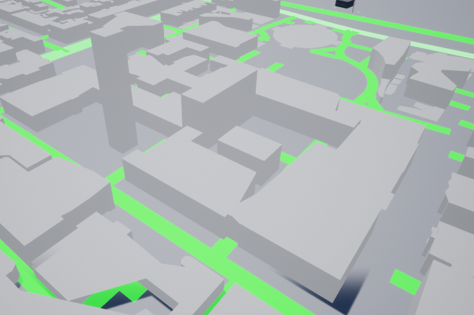
\includegraphics[width=0.5\textwidth]{04_Implementation/Map.png} 
    \caption{Source: Loaded the map of the South Kensington Campus into Unreal Engine}
    \label{StreetMapIMG}
\end{figure}